\esSezione{Cronometro su board}\label{sec:esercizio5-2}

\begin{traccia}
Sintetizzare ed implementare su board il componente sviluppato al punto precedente, utilizzando i display a 7 segmenti per la visualizzazione dell'orario (o una combinazione di display e led nel caso in cui i display a disposizione siano in numero inferiore a quello necessario), gli switch per l'immissione dell'orario iniziale e due bottoni, uno per il set dell'orario e uno per il reset. Si utilizzi una codifica a scelta dello studente per la visualizzazione dell'orario sui display (esadecimale o decimale).
\end{traccia}

\progetto

Il cronometro dell'esercizio~\ref{sec:esercizio5-1} viene mantenuto invariato (listati~\ref{lst:esercizio5-1:cronometro} e~\ref{lst:esercizio5-1:counter-mod}); il top module gli affianca quattro blocchi.

\begin{enumerate}
  \item il \texttt{debouncer}, già presentato nell'esercizio~\ref{sec:esercizio3-2} (listato~\ref{lst:esercizio3-2:debouncer}), che ripulisce il bottone centrale;
  \item l'\texttt{input\_manager}, che acquisisce ore, minuti e secondi iniziali attraverso un unico gruppo di sei switch;
  \item tre istanze di \texttt{bin2dec}, che convertono i valori binari di ore, minuti e secondi in due cifre BCD ciascuna;
  \item il \texttt{display\_driver}, che pilota in multiplexing i display a 7 segmenti e al suo interno usa il decodificatore \texttt{seg7\_decoder}.
\end{enumerate}

Per l'orario iniziale servono $5+6+6=17$ bit, più dei 16 switch della board. Si è scelto di inserire i tre campi uno alla volta, con gli stessi sei switch \texttt{SW(5:0)}, e di confermarli con una sequenza di pressioni del bottone centrale: la prima carica le ore, la seconda i minuti, la terza i secondi e genera il \texttt{set} del cronometro. I tre LED \texttt{LED(2:0)} indicano il campo in attesa di essere caricato. Il bottone inferiore \texttt{BTND} è il reset, mentre lo switch \texttt{SW(15)} è collegato all'ingresso \texttt{run} e avvia o ferma il conteggio. L'orario è mostrato in decimale su sei delle otto cifre disponibili, nella forma ore, minuti, secondi.

\implementazione

Presentiamo per primo il convertitore \texttt{bin2dec}. L'ingresso \texttt{bin} è a 6 bit (valori 0--63) e le uscite \texttt{decine} e \texttt{unita} sono due cifre BCD a 4 bit. L'architettura è \texttt{behavioral}: un process sensibile a \texttt{v}, copia unsigned di \texttt{bin}, confronta il valore con le soglie 60, 50, \ldots, 10 in una catena di \texttt{if}/\texttt{elsif}, assegna la cifra delle decine e sottrae la soglia per ottenere le unità. Così si evitano i divisori: basta un comparatore per soglia.

\vhdlfile{esercizio5-2/bin2dec.vhd}{Implementazione del convertitore binario-BCD}{lst:esercizio5-2:bin2dec}

Il decodificatore \texttt{seg7\_decoder} ha un ingresso \texttt{cifra} a 4 bit e un'uscita \texttt{seg} a 7 bit, nell'ordine \texttt{gfedcba}, attiva bassa come i segmenti della board. L'architettura \texttt{dataflow} usa un'unica assegnazione \texttt{with select}; ogni valore non compreso tra 0 e 9 spegne tutti i segmenti.

\vhdlfile{esercizio5-2/seg7_decoder.vhd}{Implementazione del decodificatore a 7 segmenti}{lst:esercizio5-2:seg7-decoder}

Il \texttt{display\_driver} ha il generic \texttt{N\_REFRESH}, di default 100\,000 cicli di clock, pari a \SI{1}{ms} a \SI{100}{MHz}. Gli ingressi sono \texttt{clk}, \texttt{rst} e le sei cifre BCD \texttt{ore\_d}, \texttt{ore\_u}, \texttt{min\_d}, \texttt{min\_u}, \texttt{sec\_d}, \texttt{sec\_u}; le uscite sono \texttt{seg} (7 bit), \texttt{dp} e \texttt{an} (8 bit), tutte attive basse. L'architettura è \texttt{structural} e riusa il contatore modulare: l'istanza \texttt{refresh} (modulo \texttt{N\_REFRESH}, 17 bit) produce un impulso \texttt{tick} ogni millisecondo, mentre \texttt{sel\_cnt} (modulo 6, 3 bit) avanza di una posizione a ogni \texttt{tick} e fornisce il segnale \texttt{sel}. Un process combinatorio, sensibile a \texttt{sel} e alle sei cifre, seleziona la cifra da mostrare, l'anodo da accendere e lo stato del punto decimale, che resta acceso sulle cifre delle unità di ore e di minuti per separare i tre campi. Un solo \texttt{seg7\_decoder} serve tutte le cifre; le due restanti non sono mai selezionate e restano spente.

\vhdlfile{esercizio5-2/display_driver.vhd}{Implementazione del Display Driver}{lst:esercizio5-2:display-driver}

L'\texttt{input\_manager} ha come ingressi \texttt{clk}, \texttt{rst}, \texttt{load} (il segnale proveniente dal debouncer) e \texttt{sw}, a 6 bit. Le uscite sono \texttt{h\_in} (5 bit), \texttt{m\_in} e \texttt{s\_in} (6 bit), l'impulso \texttt{set} e \texttt{campo} (3 bit) per i LED. L'architettura \texttt{behavioral} è una FSM a tre stati, \texttt{ORE}, \texttt{MINUTI} e \texttt{SECONDI}, descritta con un solo process sincrono: a ogni \texttt{load} il valore degli switch viene memorizzato nel registro del campo corrente e lo stato avanza; nello stato \texttt{SECONDI}, inoltre, \texttt{set} viene posto a \texttt{'1'} per un ciclo e la macchina torna in \texttt{ORE}. Il reset sincrono azzera i registri e riporta la macchina in \texttt{ORE}. L'uscita \texttt{campo} vale \texttt{"100"}, \texttt{"010"} o \texttt{"001"} a seconda dello stato.

\vhdlfile{esercizio5-2/input_manager.vhd}{Implementazione dell'Input Manager}{lst:esercizio5-2:input-manager}

Il top module \texttt{cronometro\_tl} (nel file \texttt{coronometro\_tl.vhd}) ha le porte coerenti con i nomi dei vincoli della board: \texttt{CLK100MHZ}, \texttt{SW} (16 bit), \texttt{BTNC}, \texttt{BTND}, \texttt{LED} (3 bit), i sette segmenti \texttt{CA}--\texttt{CG}, \texttt{DP} e \texttt{AN} (8 bit). L'architettura è \texttt{structural}. Il reset \texttt{rst} è collegato direttamente a \texttt{BTND}, mentre \texttt{BTNC} attraversa il \texttt{debouncer} e produce \texttt{load\_p}. Questo alimenta l'\texttt{input\_manager}, la cui uscita \texttt{set\_p} e i valori \texttt{h\_in}, \texttt{m\_in}, \texttt{s\_in} entrano nel \texttt{cronometro}, con \texttt{run} collegato a \texttt{SW(15)}. Le ore, estese a 6 bit con uno zero in testa (\texttt{h\_ext}), e i minuti e secondi passano per le tre istanze \texttt{conv\_h}, \texttt{conv\_m} e \texttt{conv\_s} di \texttt{bin2dec}; le sei cifre risultanti raggiungono il \texttt{display\_driver}. Il vettore \texttt{seg} è poi scomposto nei singoli segnali \texttt{CA}--\texttt{CG}.

\vhdlfile{esercizio5-2/coronometro_tl.vhd}{Implementazione del top module Cronometro su board}{lst:esercizio5-2:coronometro-tl}

Per questo esercizio non è stato sviluppato un testbench: il comportamento è verificato direttamente sulla scheda.

\sintesiboard

Il circuito è stato sintetizzato ed implementato sulla Nexys A7-100T. Dopo il reset con \texttt{BTND}, si impostano gli switch \texttt{SW(5:0)} sul valore delle ore e si preme \texttt{BTNC}; si ripete l'operazione per minuti e secondi, controllando sui LED il campo in corso. Alla terza pressione l'orario impostato viene caricato nel cronometro e, con \texttt{SW(15)} alto, il conteggio procede. Nella figura~\ref{fig:esercizio5-2:board} sono mostrati i display in due momenti: nella foto (a) compaiono ore, minuti e secondi con le cifre accese, nella foto (b) l'orario azzerato, con i punti decimali che separano i tre campi.

\begin{figure}[H]
  \centering
  \begin{subfigure}[b]{0.45\linewidth}
    \centering
    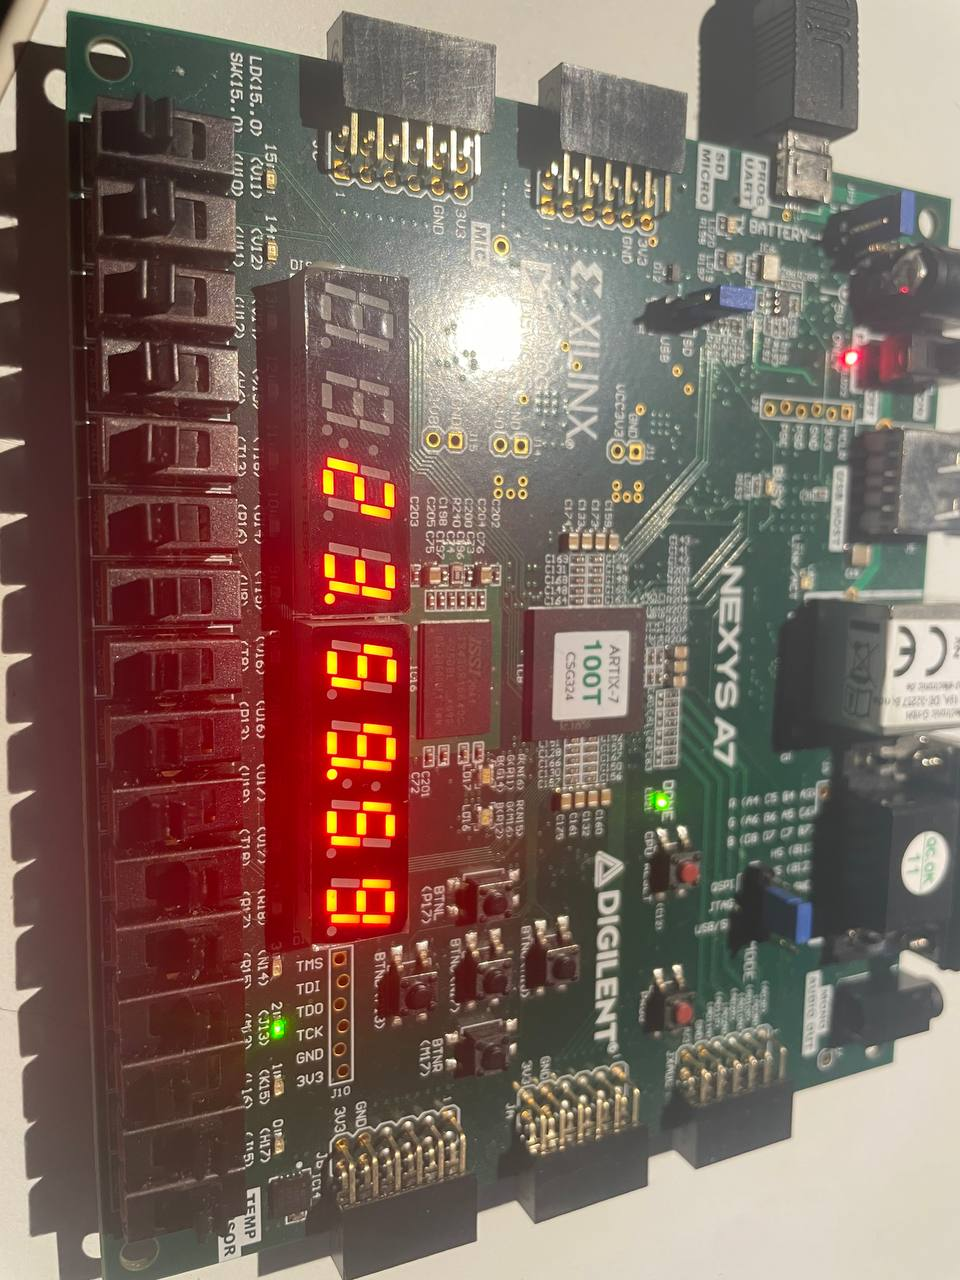
\includegraphics[width=\linewidth]{figure/esercizio5-2/board-1}
    \caption{Orario in corso}
  \end{subfigure}
  \hfill
  \begin{subfigure}[b]{0.45\linewidth}
    \centering
    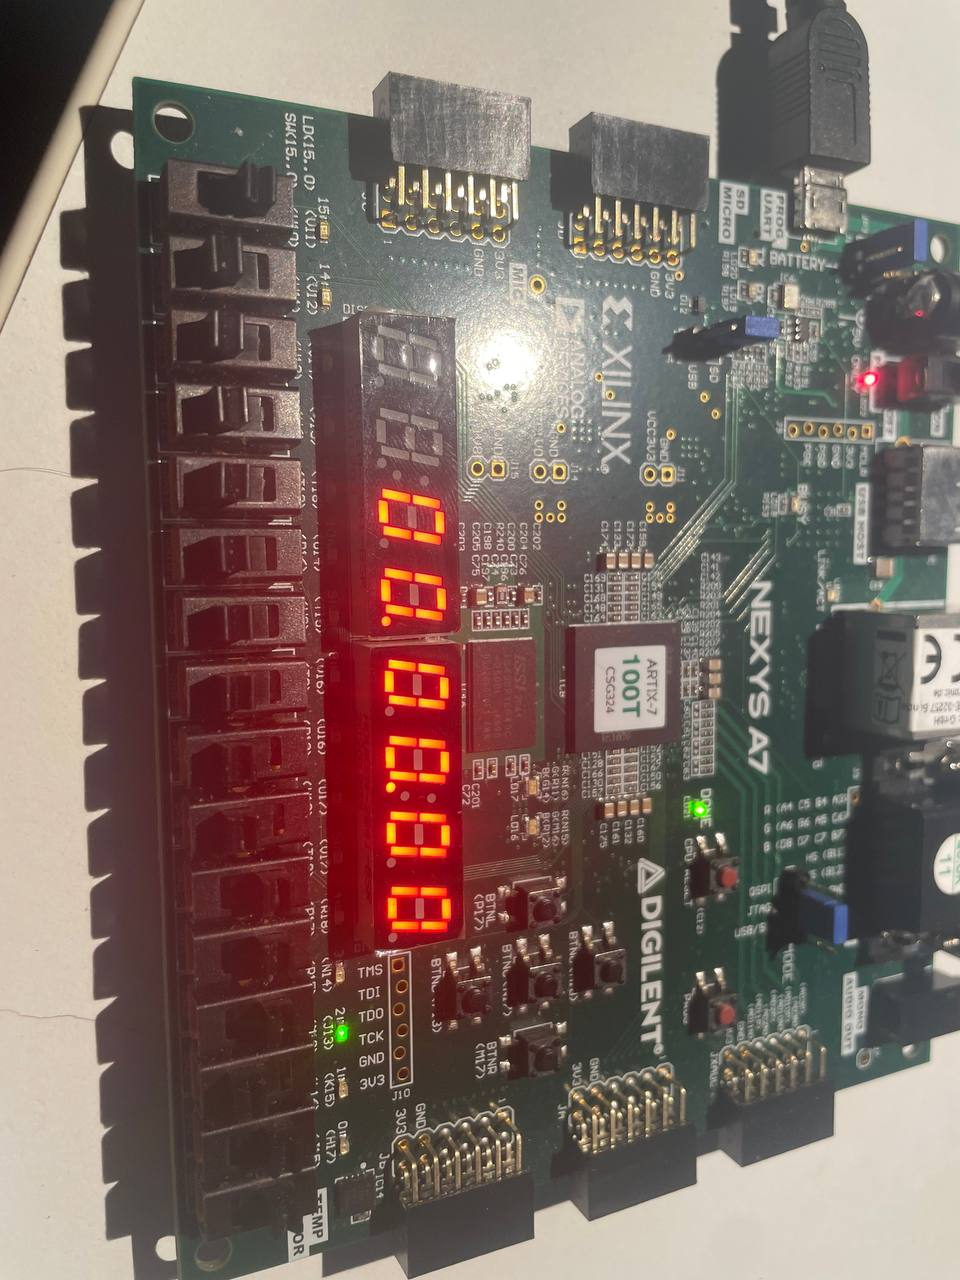
\includegraphics[width=\linewidth]{figure/esercizio5-2/board-2}
    \caption{Orario azzerato}
  \end{subfigure}
  \caption{Cronometro su Board}
  \label{fig:esercizio5-2:board}
\end{figure}

Nel file dei constraint sono state decommentate le seguenti righe.

\xdcfile{esercizio5-2/vincoli.xdc}{Constraint}{lst:esercizio5-2:vincoli}
